
With the fundamentals of probabilistic theory introduced above, we shall briefly apply this probabilistic viewpoint to establish the connection with the PES samplings [\cref{chapter:sampling_methods}] to deepen our understanding of the abstract theory of probability. 

\paragraph{\textbf{Energy model training}} We begin by examining the idea of training the energy models for atomistic simulations The basic idea is schematically illustrated with a one-dimensional toy model in \cref{fig:dummy_MC_sampling}. In an idealised scenario, we would like to compute the ground-truth potential energy function $U(x)$ [solid line in \cref{fig:dummy_MC_sampling}(a)] for a given material by solving the full many-body Schr\"{o}dinger equation, taking into account all the intricate physical interactions in that material. From here, we can easily compute the ground-truth PDF for this potential energy function as $p(x)=\exp[-\beta U(x)]$ analytically as the Boltzmann distribution[\cref{fig:dummy_MC_sampling}(b)], or through MC sampling, in which as the MC progress, we gradually build up our estimated density distribution. By computing the KL divergence of accumulated density at each MC step with respect to  $p(x)$, \cref{fig:dummy_MC_sampling}(c) shows that the KL divergence will eventually converge to zero, means the PES has been thoroughly sampled. 


\begin{figure}[tbh]
    \centering
    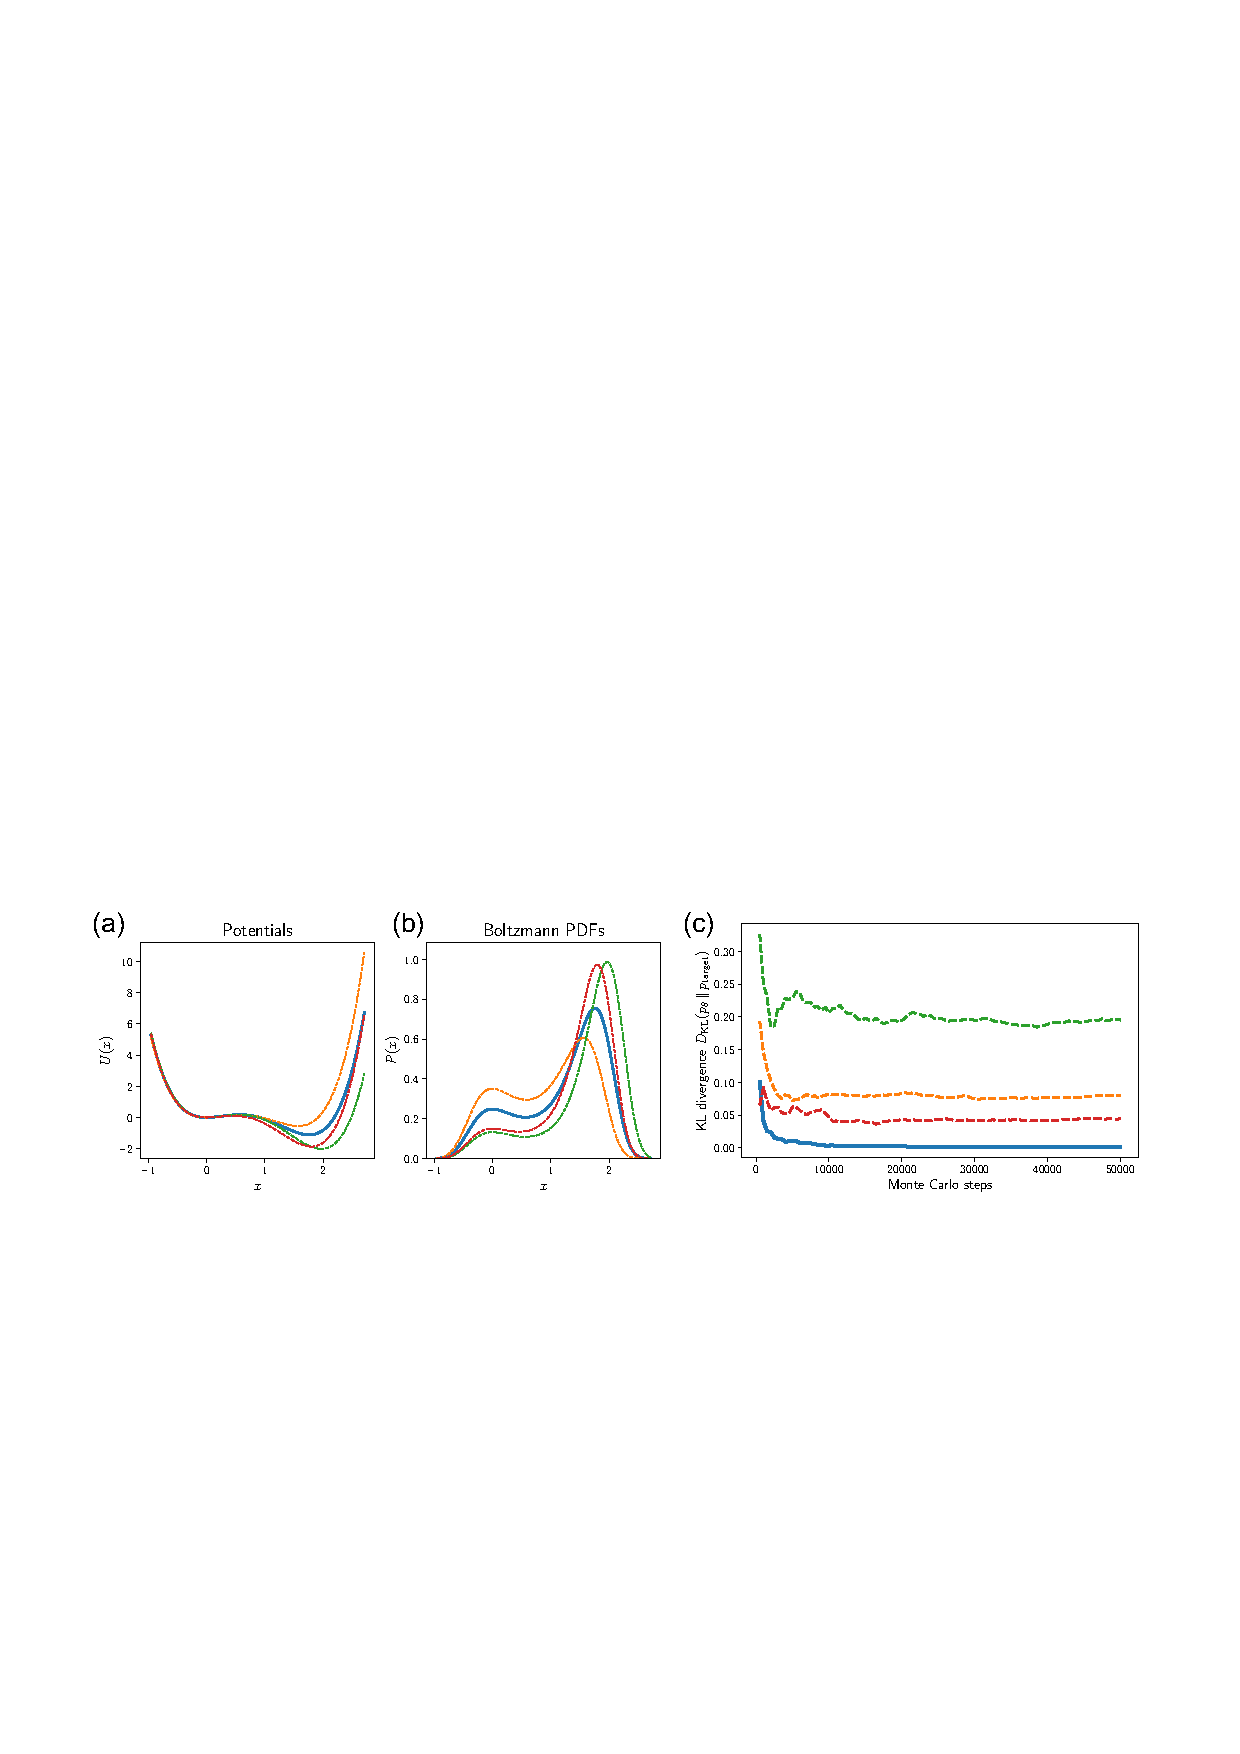
\includegraphics[width=\linewidth]{dummy_MC_sampling.pdf}
    \caption{Probabilistic view on potential energy landscape sampling using 1D toy examples. (a) Shapes for the ground-truth potential energy surface $U(x)$ (blue solid line) and its three parameterised approximations $U_\theta (x)$, mimicking either traditional or ML/AI atom-atom potentials. (b) Corresponding probability distribution functions (PDFs) for each potential as defined by the Boltzmann distribution $P(x)=e^{-\beta U(x)}$, with $\beta=1$ a.u. (c) Building the underlying PDFs for $U(x)$ and $U_\theta (x)$ with Monte Carlo (MC) sampling, which will be dubbed as $P(x)$ and $P_\theta(x)$, respectively. This plot shows the evolution of the KL divergence ($D_{KL}$ of $P(x)$ or $P_\theta(x)$ with respect to the ground-truth PDF of  $P(x)$ as a function of the MC steps. If the sampling process follows $U(x)$, then $D_{KL}$ will eventually converge to zero, whereas for samplings performed on $U_\theta(x)$, the converged $D_{KL}$ will always be greater than one, where its absolute value depends on how close $U_\theta (x)$ is to $U(x)$ in its shape.}
    \label{fig:dummy_MC_sampling}
\end{figure}



However, practically, we have to resort to some parameterised approximation $U_\theta (x)$ [dashed lines in \cref{fig:dummy_MC_sampling}(a)] to mimic the ground-truth PES $U(x)$, for example, using empirical forcefields, DFT, or ML/AI-based interatomic potentials. Correspondingly, we can also compute the approximate PDF as $p_\theta (x)=\exp[-\beta U_\theta (x)]$ [\cref{fig:dummy_MC_sampling}(b)], and perform MC sampling on this approximate PES to build up the estimated density distribution. In this case, as shown in \cref{fig:dummy_MC_sampling}(c), the KL divergence of the accumulated density with respect to the ground-truth PDF $p(x)$ will converge to a finite value greater than zero, which depends on how optimised the parameters $\theta$ are in terms of reconstructing the shape of $U(x)$ with $U_\theta (x)$. In realistic atomistic modelling, the problem of $U(x)$ being unknown is usually circumvented by using a high-level theory (such as hybrid-DFT and wavefunction method) to provide baseline or reference energies $U_{\theta}^{\mbox{\scriptsize{ref}}}(x)$ for optimising the parameters $\theta$ in $U_\theta (x)$ for lower-level approximations (such as forcefield and ML/AI models).  This is usually achieved by minimising some loss functions constructed based on $p_{\theta}^{\mbox{\scriptsize{ref}}}(x)$ and $p_\theta(x)$. In this regard, \textit{$U_{\theta}^{\mbox{\scriptsize{ref}}}(x)$ sets the `ceiling' for the accuracy that could be achieved by $U_\theta(x)$, and to what extent $x$ covers representative configurations on the PES (i.e. the size of the training set), will determine the generalisability of $U_\theta(x)$.} This is an important aspect to be mindful of when assessing the capabilities of ML/AI models.

In terms of the statistical sampling of configurations $\bm{R}$ from the PES (in which we use $\bm{R}$ here to denote the collection of all nuclear positions in the system), the probabilistic viewpoint also provides useful insights. In the language of probabilistic theory, what we would like to achieve from structural sampling is to directly draw a random variable $\bm{R}$ from some abstract space $\Omega$ that contains all possible configurations that a system might possess. The probability distribution $p(E(\bm{R}))$ of drawing $\bm{R}$ from $\Omega$ depends on the underlying potential energy model $E(\bm{R})$ and the statistical ensemble [\cref{tab:thermodynamic_ensembles}] that we are working with. 
%Under the canonical ensemble, for example, $p(U(\bm{R}))$ is given by the Boltzmann distribution as $p(U(\bm{R}))=\pi(\bm{R})= \exp[-\beta U(\bm{R})]$/\mathcal{Z}. Correspondingly, the observale is weighted over the probability distribution of $\pi(\bm{R})$, and one can rewrite \cref{eq:general_sampling_2} in the form of expectation value taken over $\pi(\bm{R})$:
%\begin{equation}
%\label{eq:general_sampling_2_expectation_val}
%\langle\mathcal{A}\rangle =\mathbb{E}_{\bm{R}\sim\pi(\bm{R})}\left[ \mathcal{A}(\bm{R})\right]=\int_{\bm{R}} \mathcal{A}(\bm{R}) \pi(\bm{R}) \mbox{d}\bm{R}.
%\end{equation}
However, since we do not have direct access to $\Omega$, $p(E(\bm{R}))$ and more importantly, the knowledge of how to inversely map the total system energy $U$ back to $\bm{R}$, we have to utilise the fundamental physics that governs the atom-atom interactions to sample the underlying PES to build up $p(E(\bm{R}))$ in traditional approach of PES sampling. On the other hand, as well shall see in \cref{sec:generative_AI}, modern generative AI models try to learn the mapping between some simple prior distributions (such as normal and uniform distributions) to $p(E(\bm{R}))$ based on large amounts of training data, and then directly draw $\bm{R}$ from $p(E(\bm{R}))$ without explicitly sampling the underlying PES. 

\paragraph{\textbf{Nested sampling and constrained MD}}
Next, we shall revisit the concepts of nested sampling and constrained MD discussed in \cref{sec:nested_sampling} in order to provide some further physical context behind the definitions of conditional and marginal probability distributions. Under the canonical ensemble, the purpose of performing PES sampling, via, \emph{e.g.} MD simulations, is to obtain the probability distribution 
\begin{equation}
    \label{eq:prob_full_sampling}
p(E(\bm{R}))=\pi(\bm{R})= \exp[-\beta E(\bm{R})]/\mathcal{Z},
\end{equation} 
from which the system entropy and free energy can be computed. To describe a chemical reaction, we shift our focus onto a subset of coordinates $\zeta\in\bm{R}$ that characterises the reaction progress, such as a bond length or dihedral angle. Further denoting $\bar{\zeta}=\bm{R}-\zeta$, the \cref{eq:prob_full_sampling} can be recasted into a form of joint probability distribution 
\begin{equation}
    \label{eq:joint_prob_full_sampling}
\pi(\zeta,\bar{\zeta})= \exp[-\beta E(\zeta,\bar{\zeta})]/\mathcal{Z}.
\end{equation} 
From here, the free energy profile along the reaction coordinate $\zeta$ can be computed via the marginal probability distribution
\begin{equation}    
\label{eq:marginal_prob_sampling}
\pi(\zeta)=\int \pi(\zeta,\bar{\zeta}) \mbox{d}\bar{\zeta}
\end{equation}
Determining this integrand can be achieved through constrained molecular dynamics, which effectively samples the conditional probability distribution $\pi(\zeta|\bar{\zeta})$ that leads to the integrand $\langle \partial\mathcal{H}/\partial {\zeta}\rangle_{\zeta^\prime}^{\mbox{\scriptsize{cond.}}}$ in \cref{eq:thermodynamic_integration}.\footnote{To show this, we start from the marginal probability distribution
$
    \pi(\zeta)=\frac{1}{\mathcal{Z}}\int\exp\left[-\beta E(\zeta,\bar{\zeta})\right]\mbox{d}\bar{\zeta},
$
differentiate both sides with respect to $\zeta$ gives
$
    \frac{\partial\pi(\zeta)}{\partial\zeta}=\frac{1}{\mathcal{Z}}\int\left(-\beta\frac{\partial E(\zeta,\bar{\zeta})}{\partial \zeta}\right)\exp\left[-\beta E(\zeta,\bar{\zeta})\right]\mbox{d}\bar{\zeta},
$
and 
$
    \frac{1}{\pi(\zeta)}\frac{\partial\pi(\zeta)}{\partial\zeta}=-\beta\int\frac{1}{\pi(\zeta)}\frac{e^{-\beta E(\zeta,\bar{\zeta})}}{\mathcal{Z}}\left(-\frac{\partial E(\zeta,\bar{\zeta})}{\partial \zeta}\right)\mbox{d}\bar{\zeta}.
$
Now using the relationship 
$
\pi(\bar{\zeta}|\zeta)=\frac{\pi(\zeta,\bar{\zeta})}{\pi(\zeta)}=\frac{1}{\pi(\zeta)}\frac{\exp\left[-\beta E(\zeta,\bar{\zeta})\right]}{\mathcal{Z}}
$
such that 
$
    \frac{1}{\pi(\zeta)}\frac{\partial\pi(\zeta)}{\partial\zeta}=-\beta\int\pi(\bar{\zeta}|\zeta) \frac{\partial E(\zeta,\zeta^\prime)}{\partial \zeta}\mbox{d}\zeta^\prime=-\beta\left\langle \frac{\partial E}{\partial\zeta}\right\rangle_{\zeta^\prime},
$
by using the definition of expectation value.
}


\paragraph{\textbf{(Information) entropy for a simple quantum harmonic oscillator}}
As the third example, we examine the definition of information entropy [\cref{eq:information_entropy}]. To put such definition into a more physical context, and establish its linkage to the concept of entropy in statistical physics, we consider the problem of vibrational entropy of a simple quantum harmonic oscillator. For this simple physical system, its energy eigenspectrum is $E_n=\left(n+\frac{1}{2}\right)\hbar\omega$, with $\omega$ being the characteristic frequency and $n=0,1,2,\ldots$. This gives the probability distribution function $p_n=\exp\left[-\beta\hbar\omega \left(n+\frac{1}{2}\right)\right]/\mathcal{Z}$ for finding an oscillator in its $n$-th quantum state, with the partition function 
\begin{equation*}
    \mathcal{Z}=\sum_{n=0}^{\infty}\exp\left[-\beta\hbar\omega \left(n+\frac{1}{2}\right)\right]=e^{-\beta\hbar\omega/2}\left(1-e^{-\beta\hbar\omega}\right),
\end{equation*}
that can be easily determined as the infinite sum of a converged geometric series. This leads to
\begin{equation*}
    p_n =\left(1-e^{-\beta\hbar\omega}\right)e^{-n\beta\hbar\omega}.
\end{equation*}
In statistical mechanics, the entropy for a system with microstate $i$ and probability $p_i$ [equivalent to \cref{eq:information_entropy}] is 
\begin{equation}
    \label{eq:entropy_stat_mech}
    S=-k_B\sum_i p_i\ln p_i.
\end{equation}
To simplify the notations, by letting $q=e^{-\beta\hbar\omega}$, we have $p_n=(1-q)q^n$, and $\ln p_n=\ln(1-q)+n\ln q$, we obtain the following alternative form for \cref{eq:entropy_stat_mech}:
\begin{equation}
    \label{eq:entropy_stat_mech_har_oscillator}
    S=-k_B\sum_n \left(p_n\ln (1-q)+np_n\ln q\right)=-k_B[\ln(1-q)+\langle n\rangle q],
\end{equation}
in which we have used the fact that $\sum_n p_n=1$ (the normalisation condition) and $\sum_n np_n=\langle n\rangle =\left[e^{\beta\hbar\omega}-1\right]^{-1}=q/(1-q)$ (expected number of excited oscillator at $T$). The latter expression gives $q=\langle n\rangle/(\langle n\rangle +1)$, which, upon substituting into \cref{eq:entropy_stat_mech_har_oscillator}, leads to the final expression for the entropy:
\begin{equation}
    \label{eq:entropy_stat_mech_har_oscillator_n}
    S=k_B\left[ (\langle n\rangle+1)\ln(\langle n\rangle+1) -\langle n\rangle \ln\langle n\rangle\right].
\end{equation}
It is not difficult to prove that $S$ is a monotonically increasing function of the expectation value $\langle n\rangle$ as given by \cref{eq:entropy_stat_mech_har_oscillator_n}, which means that at large $\langle n\rangle$ (or high temperature), more vibrational modes will get excited. Consequentially, it become less uncertain on exactly which mode(s) is excited at $T$, resulting in a higher vibrational (or information) entropy in the system.

\paragraph{\textbf{Probabilistic interpretation of vibrational anharmonicity measure}}
Finally, we provide the derivation here to showcase how  the vibrational anharmonicity score,\cite{knoop2020anharmonicity} originally defined based on the ratio between the standard deviations of anharmonic and total atomic forces [\cref{eq:anharmonic_score}], can be equivalently defined in terms of KL-diverges [\cref{eq:KL_divergence}] between two probability distributions and interpreted accordingly. For simplicity, we derive the analytical expressions for the anharmonic scores based on a simple form of one-dimensional anharmonic potential in the form of $U(x)=kx^2+k^{\prime}x^3$. 

We begin by first following the original definition of the anharmonicity score based on the standard deviation of the forces, in which we decompose the total atomic force $F_{\mbox{\scriptsize{tot}}}(x)$ into the sum of the harmonic $F_{\mbox{\scriptsize{harm}}}(x)=-2kx$ and anharmonic $F_{\mbox{\scriptsize{anh}}}(x)=-3k^{\prime}x^2$ components. Furthermore, we assume  $k\gg k^{\prime}$ such that we can treat the anharmonic force as a perturbation to the harmonic component. For the harmonic reference potential $U_{\mbox{\scriptsize{harm}}}(x)=kx^2$, the corresponding probability distribution is a Gaussian $p_0 (x)=\exp\left(-\beta kx^2\right)$. We know that for a standard Gaussian distribution $\mathcal{N}(x|0,\sigma^2)$, the expectation values for the moments of $x$ follows $\left\langle x^{2n}\right\rangle=\frac{(2n)!}{2^n\cdot n!}\sigma^{2n}$ and $\left\langle x^{2n+1}\right\rangle=0$ ($n\in\mathbb{Z}$ and $n\geq 0$), so for the probability distribution $p_0(x)$, we have the following:
\begin{equation*}
    \langle x\rangle_0=0,\quad \left\langle x^2\right\rangle_0=\frac{1}{2k\beta},\qquad \left\langle x^3\right\rangle_0=0,\qquad\left\langle x^4\right\rangle_0=\frac{3}{4\beta^2k^2}.
\end{equation*}
From here, one has the following expression for the variance for the harmonic force
\begin{equation} 
\label{eq:variance_F_harm}
\mbox{Var}\left(F_{\mbox{\scriptsize{harm}}}\right)=\left\langle F_{\mbox{\scriptsize{harm}}}^2\right\rangle-\left\langle F_{\mbox{\scriptsize{harm}}}\right\rangle^2=\left\langle F_{\mbox{\scriptsize{harm}}}^2\right\rangle=4k^2\left\langle x^2\right\rangle=\frac{2k}{\beta},
\end{equation}
using the fact that $\left\langle F_{\mbox{\scriptsize{harm}}}\right\rangle\sim\langle x\rangle_0=0$. Similarly, for the anharmonic force, its variance is 
\begin{equation}
    \label{eq:variance_F_anh}
    \mbox{Var}\left(F_{\mbox{\scriptsize{anh}}}\right)=9k^{\prime 2}\left[\langle x^4\rangle-\left(\langle x^2\rangle\right)^2\right]=\frac{9k^{\prime 2}}{2\beta^2k^2}=\frac{9}{4}\lambda\cdot\mbox{Var}\left(F_{\mbox{\scriptsize{harm}}}\right),
\end{equation}
in which we have defined $\lambda=k^{\prime 2}/(\beta k^2)$. Using the fact that $\mbox{Cov}(F_{\mbox{\scriptsize{harm}}},F_{\mbox{\scriptsize{anh}}})=0$, we can combine \cref{eq:variance_F_harm} and \cref{eq:variance_F_anh} to get the variance in the total atomic force being
\begin{equation}
    \label{eq:variance_F_total}
\mbox{Var}\left(F_{\mbox{\scriptsize{tot}}}\right)=\mbox{Var}\left(F_{\mbox{\scriptsize{harm}}}\right)+\mbox{Var}\left(F_{\mbox{\scriptsize{anh}}}\right)=\left(1+\frac{9}{4}\lambda\right)\mbox{Var}\left(F_{\mbox{\scriptsize{harm}}}\right),
\end{equation}
which by combining with \cref{eq:variance_F_anh}, we arrive at the following analytical expression for the anharmonicity score for this simple one-dimensional anharmonic potential:
\begin{equation}
    \label{eq:anh_score_1D_from_variance}
    \sigma^{(2)}=\sqrt{\frac{\mbox{Var}\left(F_{\mbox{\scriptsize{anh}}}\right)}{\mbox{Var}\left(F_{\mbox{\scriptsize{tot}}}\right)}} =\sqrt{\frac{\frac{9}{4}\lambda}{\left(1+\frac{9}{4}\lambda\right)}}\approx\frac{3}{2}\sqrt{\lambda},
\end{equation}
at the weak anharmonic limit ($k^\prime\ll k)$. To derive the similar result based on the definition of KL-divergence, we can re-use the results above and approximate the distributions of anharmonic and total forces as Gaussian distributions, \emph{i.e.}, $p_{\mbox{\scriptsize{anh}}}(F)\approx\mathcal{N}(0,\sigma_{\mbox{\scriptsize{anh}}}^2)$ and $p_{\mbox{\scriptsize{tot}}}(F)\approx\mathcal{N}(0,\sigma_{\mbox{\scriptsize{tot}}}^2)$, with $\sigma_{\mbox{\scriptsize{anh}}}^2/\sigma_{\mbox{\scriptsize{tot}}}^2=\left[\sigma^{(2)}\right]^2=u(\lambda)$. By using the analytical expression of the KL-divergence between two Gaussian distributions, we then have
\begin{equation}
    \label{eq:KL_div_anh_tot}
    \mathcal{D}_{KL}\left(p_{\mbox{\scriptsize{anh}}}||p_{\mbox{\scriptsize{tot}}}\right)=\frac{1}{2}\left[\frac{\sigma_{\mbox{\scriptsize{anh}}}^2}{\sigma_{\mbox{\scriptsize{tot}}}^2}-\ln\left(\frac{\sigma_{\mbox{\scriptsize{anh}}}^2}{\sigma_{\mbox{\scriptsize{tot}}}^2}\right)-1\right]
    =\frac{1}{2}\left[u(\lambda) -\ln u(\lambda)-1\right],
\end{equation}
which shows that $\mathcal{D}_{KL}$ is a monotonically decreasing function of the anharmonicity score in the region of $\sigma^{(2)}\in[0,1]$. This shows that, for example, in the limit of $k^\prime\to0$ (or small $\sigma^{(2)}$, the potential $U(x)$ is dominated by the harmonic part, such that $p(F_{\mbox{\scriptsize{anh}}})$ differs significantly from $p(F_{\mbox{\scriptsize{tot}}})$, leading to a large  $\mathcal{D}_{KL}$, and \emph{vice versa}. This completes our derivation of anharmonic scores from the perspective of KL-divergence between two probability distributions. 